\chapter{Resultados y Análisis}\label{chapter:results}

\todopaused{RESULTADOS: Escribir cuando existan}
\todoimprove{Revisar pruebas de eficiencia de Stachowicz~\cite{Stachowicz2012}, y Vijayakumar~\cite{Vijayakumar2014}. Agregar referencia a sus evaluaciones.}
\todoimprove{Revisar pruebas de escalabilidad de Stachowicz~\cite{Stachowicz2012}, y Vijayakumar~\cite{Vijayakumar2014}. Agregar referencia a sus evaluaciones.}


\section{Consideraciones}

\todowrite{Sobre las consultas}
\todowrite{Colores de consultas}
\todowrite{Sobre CPM}
\todowrite{Estimaciones}
\todowrite{Corregir Anexo con validacioens}
\todowrite{Captions y tamaños de figuras}


% Sobre máquinas de estado para validaciones de funcionalidad


\subsection{Mediciones de eficiencia y escalabilidad}
% Mediciones eficiencia y escalabilidad
% - sobre su ejecución y generación de gráficos. 
% - sobre Tiempo de pruebas
% - sobre metodología de medición: 
%   - cada operación medida fue repetida N veces. 
%   - Se agregan árboles aleatorios de 20 episodios (tamaño esperado) y profundidad 3.
%   - Las consultas son XX. Para evitar que MongoDB cachee las respuestas y así afectar los resultados, cada campo de consulta es generado aleatóriamente entre ~1000 valores posibles.
% - Sobre las consideraciones de las pruebas:
%   - Servidor LTM: Corre en 1 CPU, a menos que los plugins implementados por el usuario sean multithread.
%   - Servidor MongoDB: Corre en 1 CPU.
% Sobre la Máquina donde se probó la cosa. Disco, IO, RAM, CPU


\section{Validaciones de Escalabilidad}

\begin{figure}[H]
	\centering
	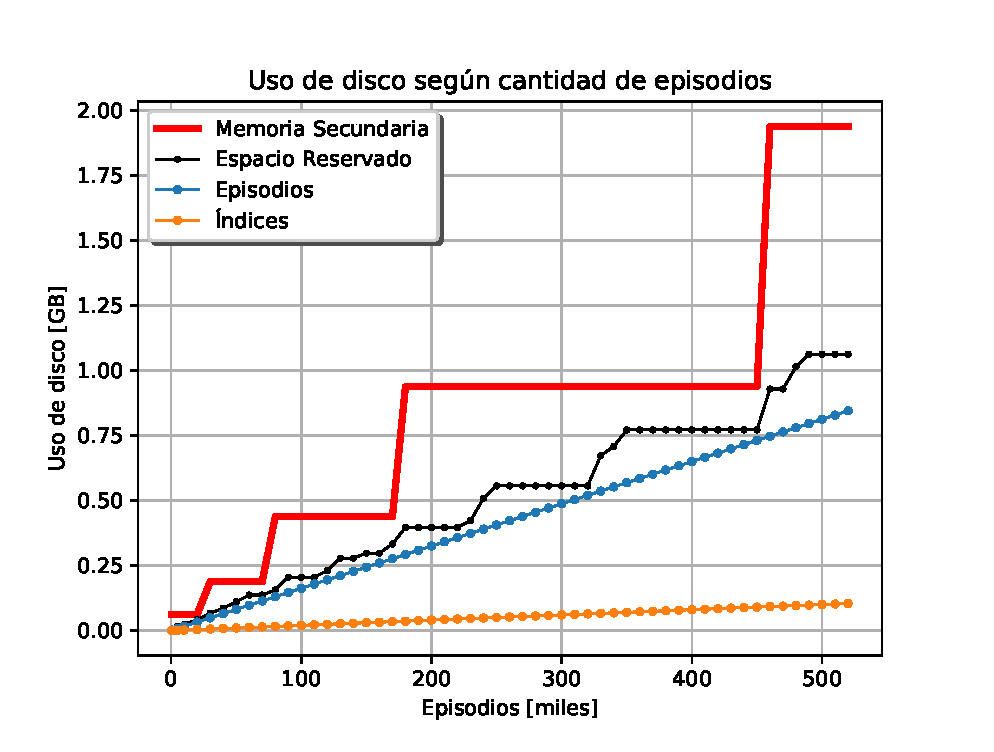
\includegraphics[width=0.65\textwidth]{results/scalability_disk_usage.eps}
	\caption[]
	{\small }
	\label{img:result_scalability_disk_usage}
\end{figure}


\begin{figure}[H]
	\centering
	\begin{subfigure}[b]{0.65\textwidth}
		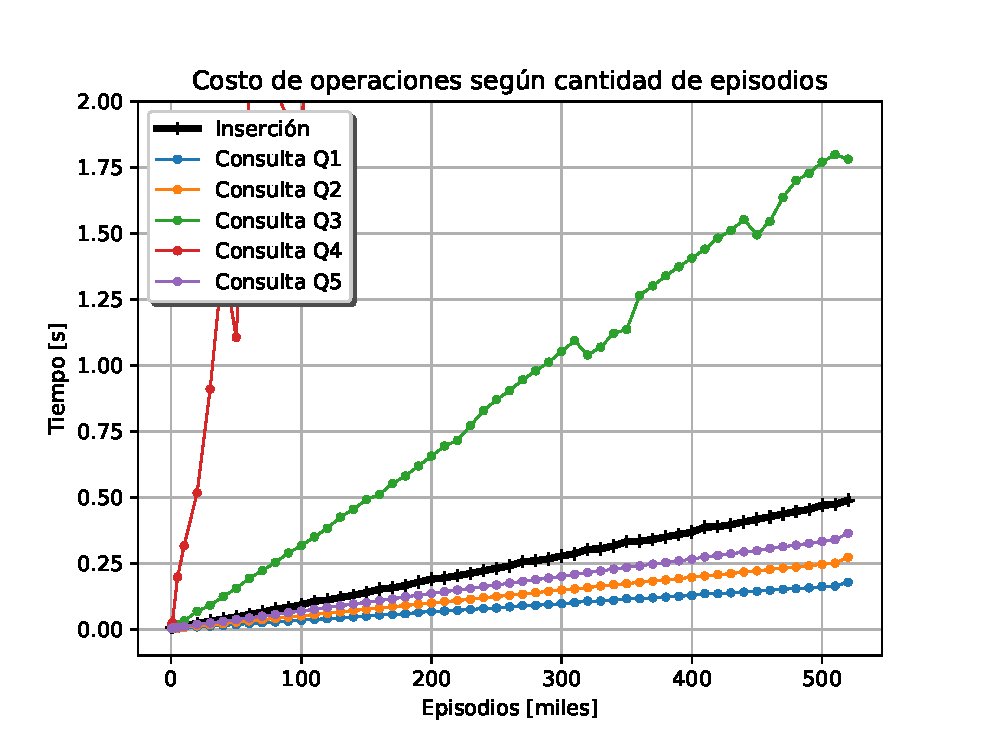
\includegraphics[width=\textwidth]{results/scalability_operation_time.eps}
		\caption{V1}
		\label{fig:gull}
	\end{subfigure}
	~
	\begin{subfigure}[b]{0.65\textwidth}
		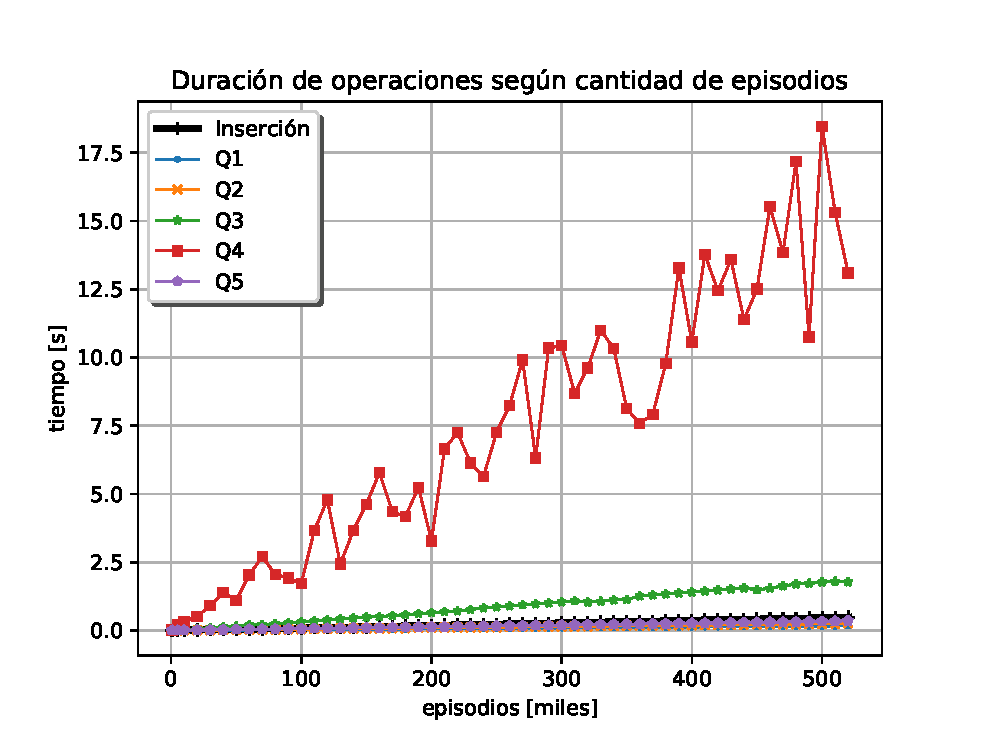
\includegraphics[width=\textwidth]{results/scalability_operation_time_extended.eps}
		\caption{Versión extendida}
		\label{fig:tiger}
	\end{subfigure}
	\caption[Escalabilidad: Duración de consultas según cantidad de episodios.]
	{\small Escalabilidad: Duración de consultas según cantidad de episodios.}\label{fig:animals}
\end{figure}

\begin{figure}[H]
	\centering
	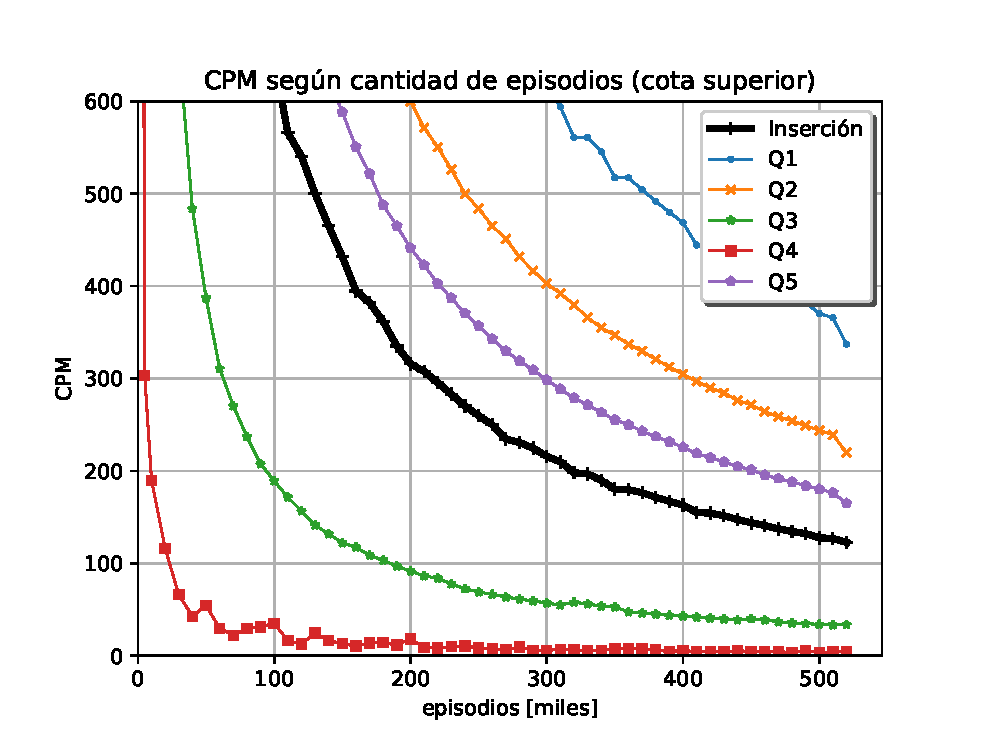
\includegraphics[width=0.65\textwidth]{results/scalability_max_qpm.eps}
	\caption[]
	{\small }
	\label{img:result_scalability_max_qpm}
\end{figure}


\section{Validaciones de Eficiencia}

\begin{figure}[H]
	\centering
	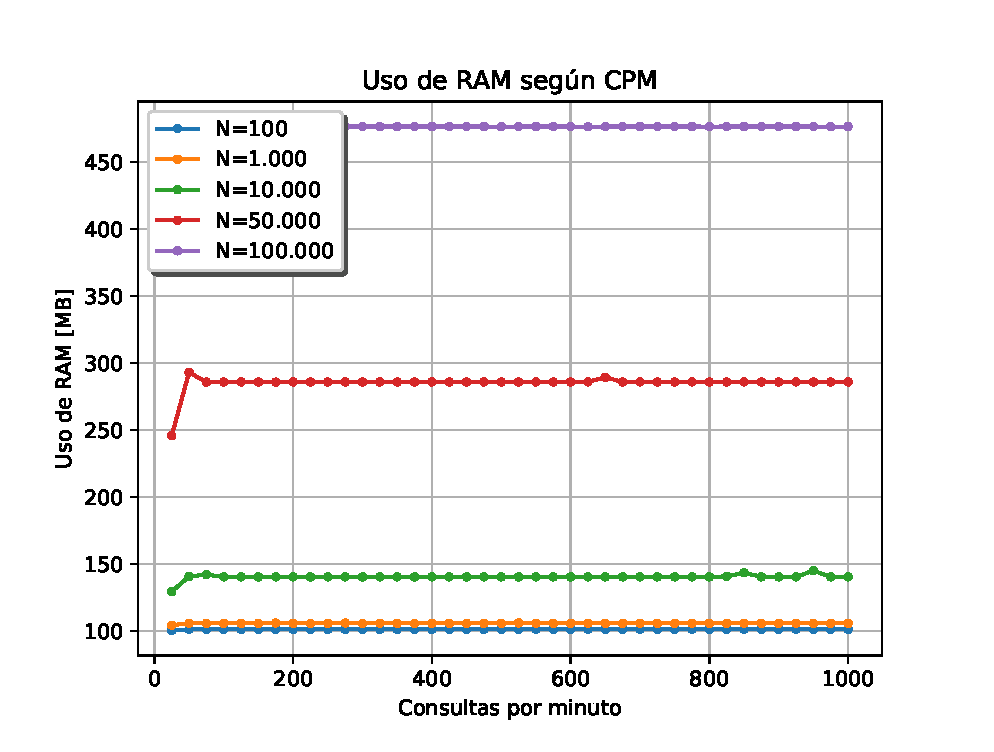
\includegraphics[width=0.65\textwidth]{results/eff__ram_qpm.eps}
	\caption[]
	{\small }
	\label{img:result_eff__ram_qpm}
\end{figure}

\subsection{Uso de CPU vs CPM by Q, EP fijo}

\begin{figure}[H]
	\centering
	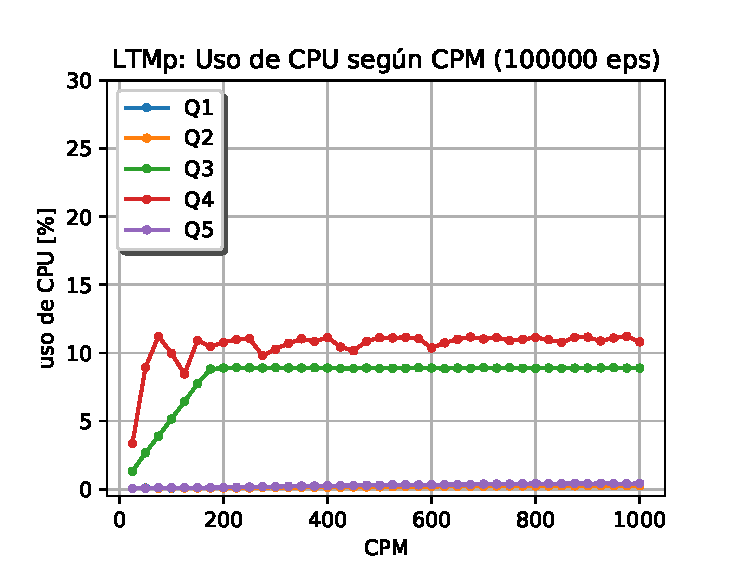
\includegraphics[width=0.8\textwidth]{results/eff__cpu_qpm_by_query__ltm__100000_episodes.eps}
	\caption[]
	{\small }
	\label{img:result_eff__cpu_qpm_by_query__ltm__100000_episodes}
\end{figure}
\begin{figure}[H]
	\centering
	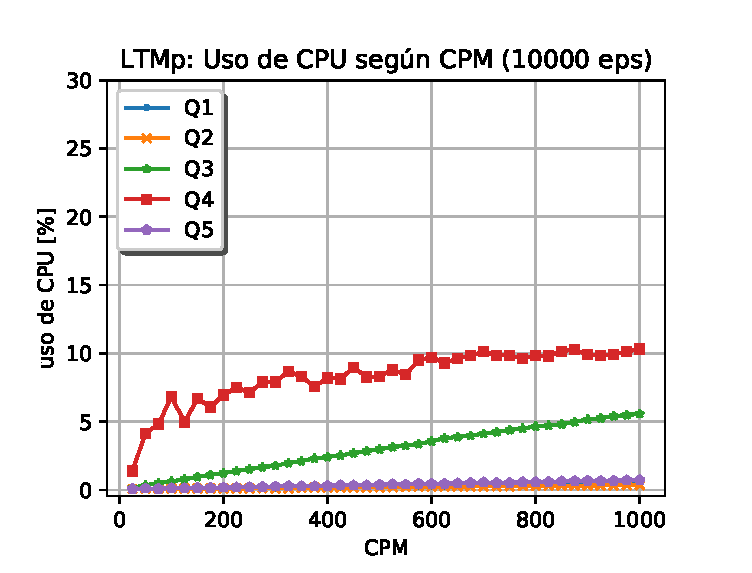
\includegraphics[width=0.8\textwidth]{results/eff__cpu_qpm_by_query__ltm__10000_episodes.eps}
	\caption[]
	{\small }
	\label{img:result_eff__cpu_qpm_by_query__ltm__10000_episodes}
\end{figure}
\begin{figure}[H]
	\centering
	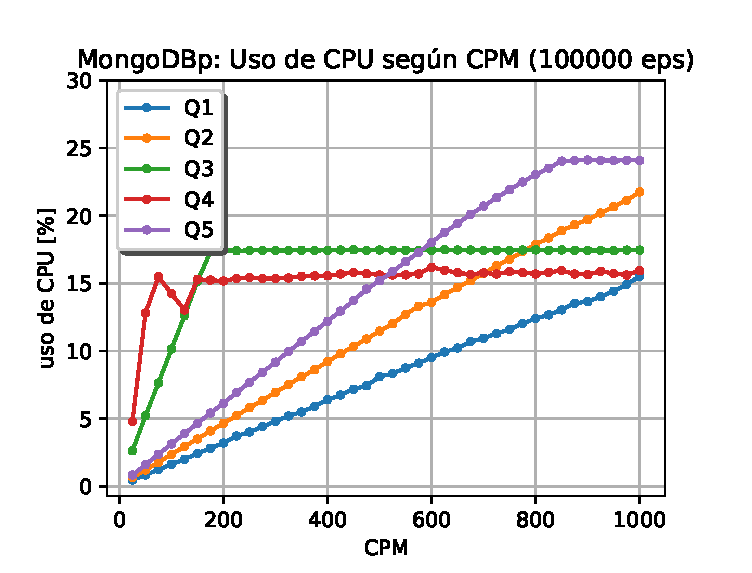
\includegraphics[width=0.8\textwidth]{results/eff__cpu_qpm_by_query__mongo__100000_episodes.eps}
	\caption[]
	{\small }
	\label{img:result_eff__cpu_qpm_by_query__mongo__100000_episodes}
\end{figure}
\begin{figure}[H]
	\centering
	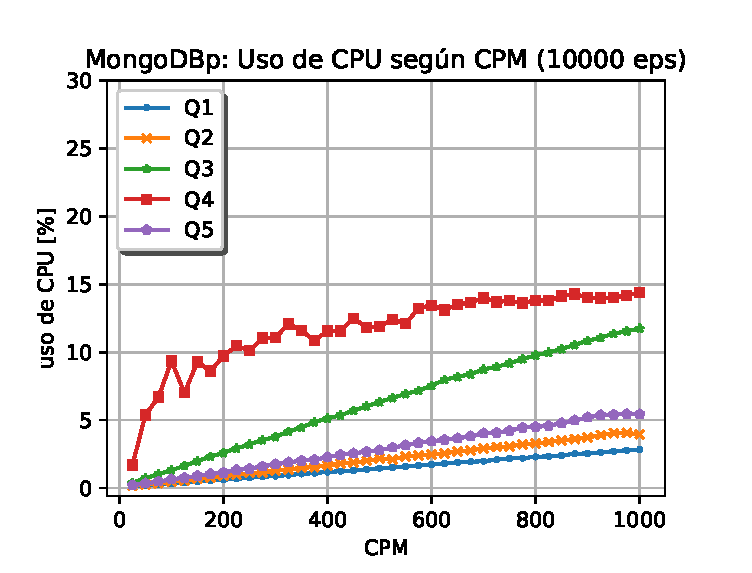
\includegraphics[width=0.8\textwidth]{results/eff__cpu_qpm_by_query__mongo__10000_episodes.eps}
	\caption[]
	{\small }
	\label{img:result_eff__cpu_qpm_by_query__mongo__10000_episodes}
\end{figure}
\begin{figure}[H]
	\centering
	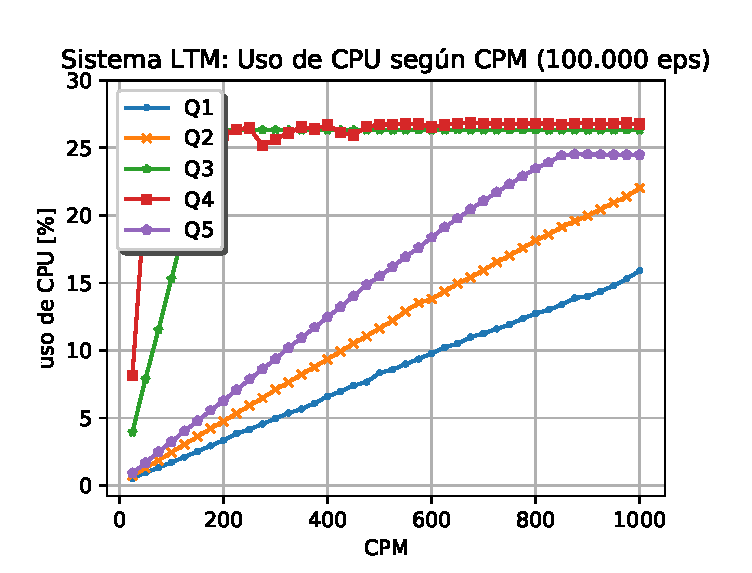
\includegraphics[width=0.8\textwidth]{results/eff__cpu_qpm_by_query__sum__100000_episodes.eps}
	\caption[]
	{\small }
	\label{img:result_eff__cpu_qpm_by_query__sum__100000_episodes}
\end{figure}
\begin{figure}[H]
	\centering
	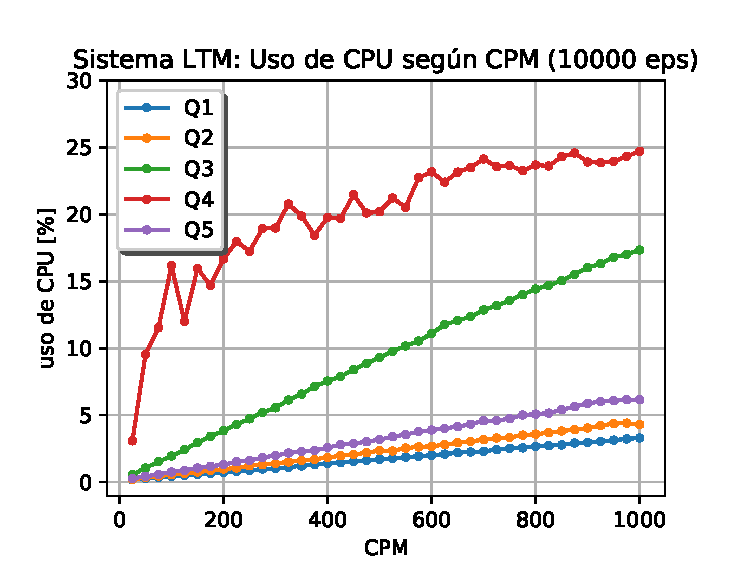
\includegraphics[width=0.8\textwidth]{results/eff__cpu_qpm_by_query__sum__10000_episodes.eps}
	\caption[]
	{\small }
	\label{img:result_eff__cpu_qpm_by_query__sum__10000_episodes}
\end{figure}

\subsection{Uso de CPU vs CPM by EPS, Q fijo}


\begin{figure}[H]
	\centering
	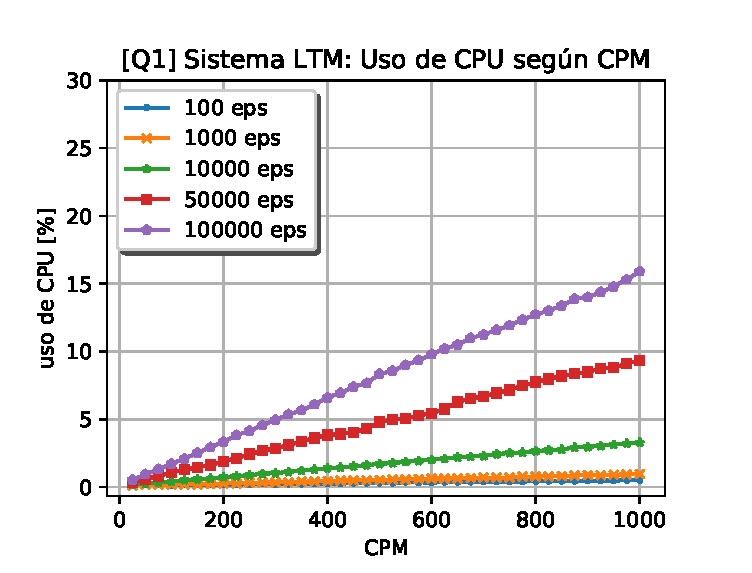
\includegraphics[width=0.8\textwidth]{results/eff_cpu_qpm_by_eps__sum__q1.eps}
	\caption[]
	{\small }
	\label{img:result_eff_cpu_qpm_by_eps__sum__q1}
\end{figure}
\begin{figure}[H]
	\centering
	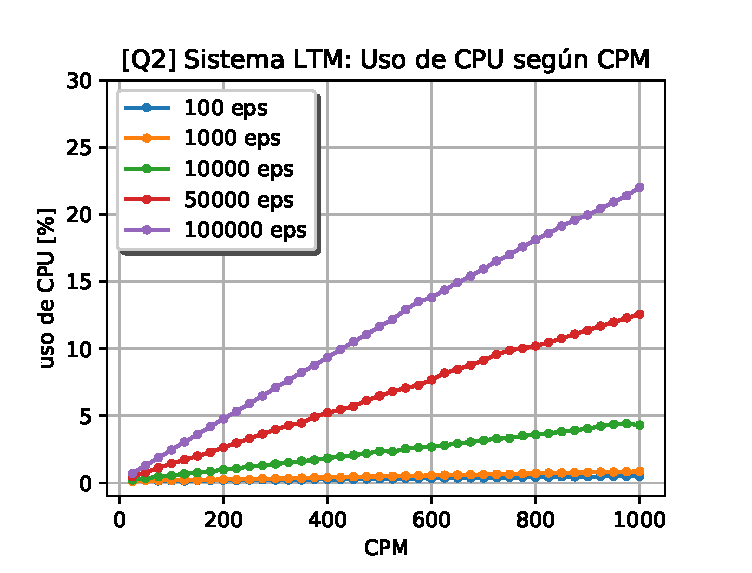
\includegraphics[width=0.8\textwidth]{results/eff_cpu_qpm_by_eps__sum__q2.eps}
	\caption[]
	{\small }
	\label{img:result_eff_cpu_qpm_by_eps__sum__q2}
\end{figure}
\begin{figure}[H]
	\centering
	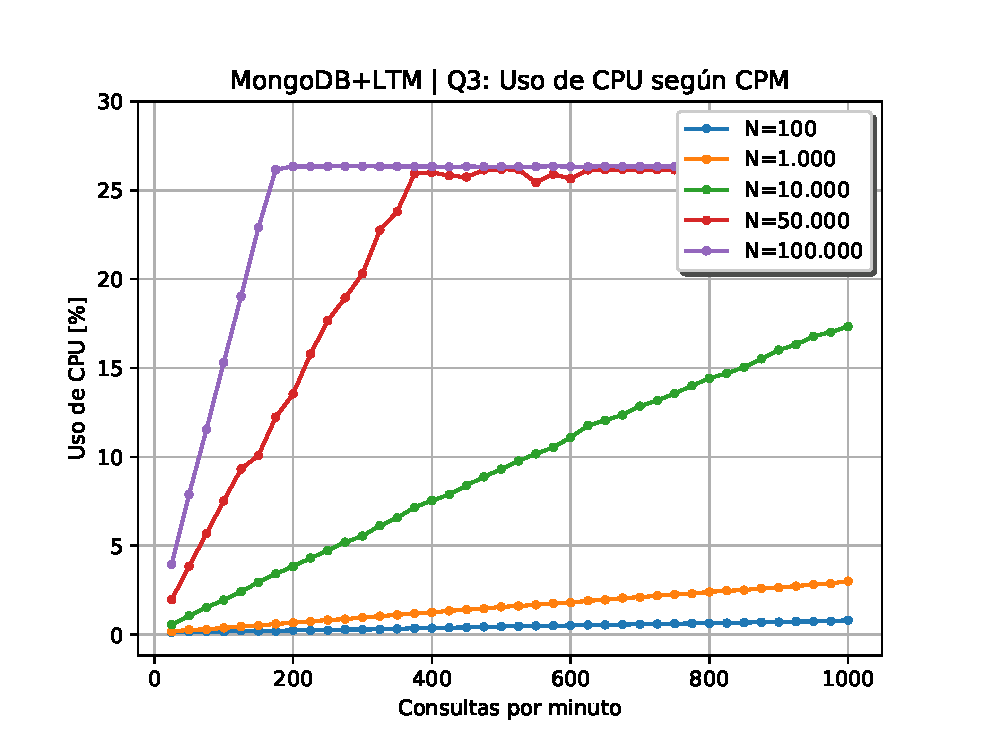
\includegraphics[width=0.8\textwidth]{results/eff_cpu_qpm_by_eps__sum__q3.eps}
	\caption[]
	{\small }
	\label{img:result_eff_cpu_qpm_by_eps__sum__q3}
\end{figure}
\begin{figure}[H]
	\centering
	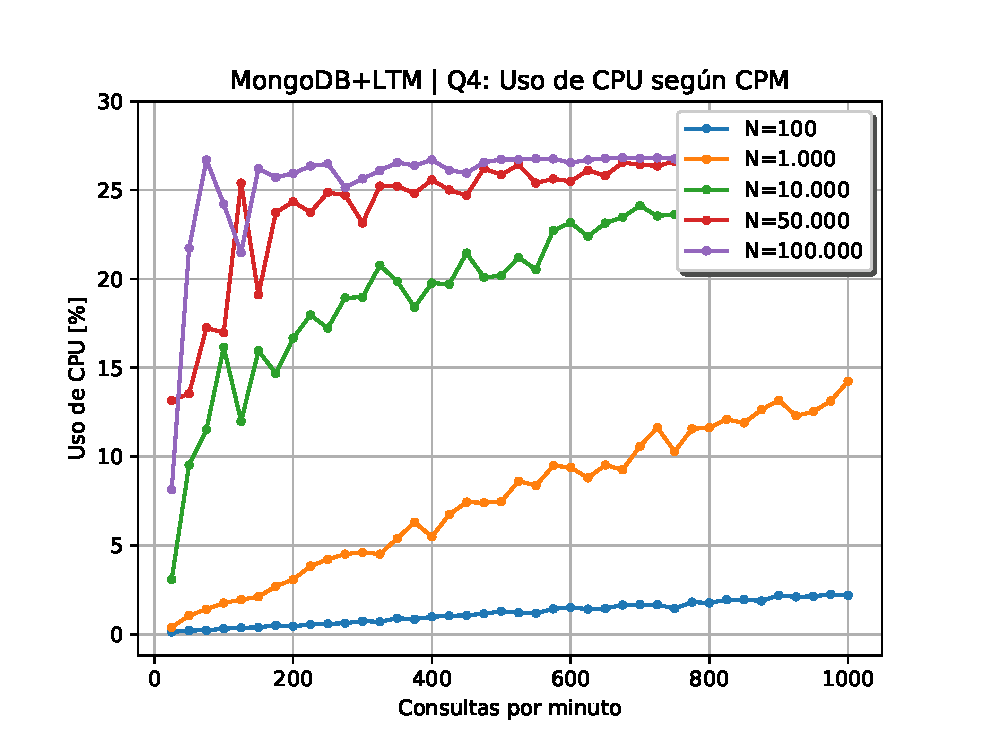
\includegraphics[width=0.8\textwidth]{results/eff_cpu_qpm_by_eps__sum__q4.eps}
	\caption[]
	{\small }
	\label{img:result_eff_cpu_qpm_by_eps__sum__q4}
\end{figure}
\begin{figure}[H]
	\centering
	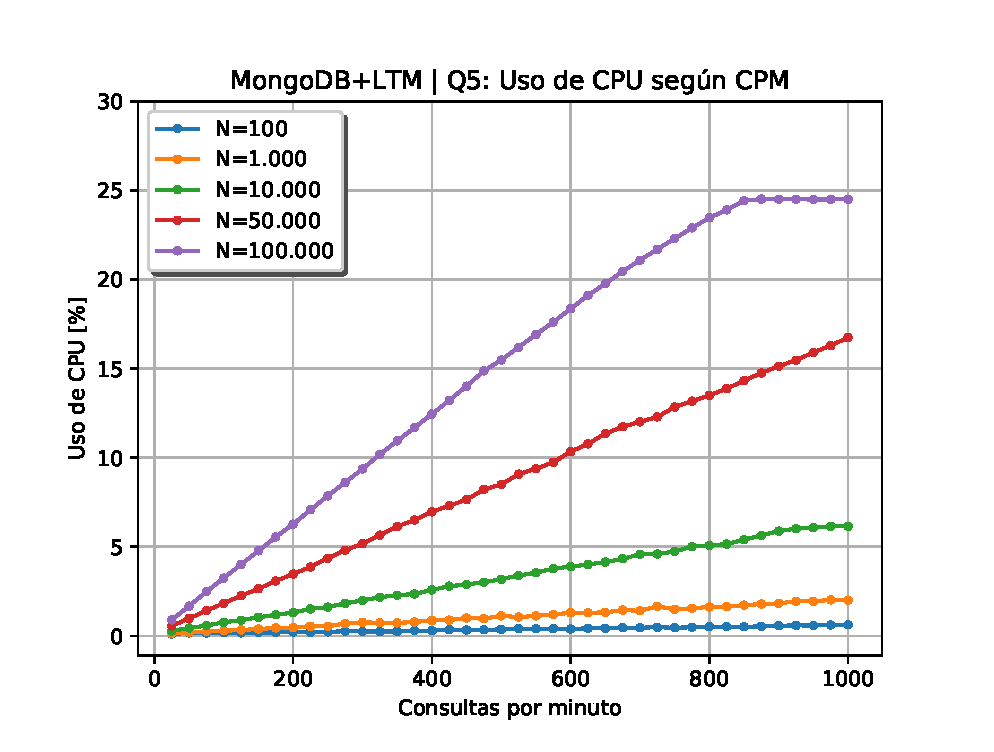
\includegraphics[width=0.8\textwidth]{results/eff_cpu_qpm_by_eps__sum__q5.eps}
	\caption[]
	{\small }
	\label{img:result_eff_cpu_qpm_by_eps__sum__q5}
\end{figure}


\section{Otras Validaciones}

% - 
% - 
% - 
